\listfiles
\documentclass[%
 reprint,%
%secnumarabic,%
 amssymb, amsmath,%
 aip,cha,%
%groupedaddress,%
%frontmatterverbose,
]{revtex4-1}

\usepackage{docs}%
\usepackage{bm}%
\usepackage{mathtools}
\usepackage{graphicx}
\usepackage[colorlinks=true,linkcolor=blue]{hyperref}%
%\nofiles
\expandafter\ifx\csname package@font\endcsname\relax\else
 \expandafter\expandafter
 \expandafter\usepackage
 \expandafter\expandafter
 \expandafter{\csname package@font\endcsname}%
\fi
\hyphenation{title}

\begin{document}

\title{Streak Camera System and Tune Resonance Tool}%

\author{L. Dovlatyan, M. Ries, P. Goslawski, and friends at HZB}%
\email{levondov@berkeley.edu}
\affiliation{University of California Berkeley,94720 Berkeley, CA, USA}%

\date{August 2014}%
%\revised{August 2010}%

\maketitle

\tableofcontents

\section{Introduction}

The Helmholtz-Zentrum Berlin is a facility that operates two synchrotron light sources: BESSY II and the MLS. One of the long term goals of this center is to continually make bunch lengths as short as possible in storage rings. A way to go about this is through lattice design by changing the momentum compaction factor. An important part of lattice design involves picking a good working point to avoid the tune resonances of the machine. A tune resonance program was therefore developed which can be used to view the current working point and resonance lines given only a few input parameters from the EPICS control systems.

Another way of looking into bunch lengths at HZB is through diagnostic tools. A new streak camera was recently purchased for the MLS, and is currently being setup and tested. The Metrology Light Source (MLS) is an electron storage ring designed as a dedicated UV and VUV source; it has an asymmetric double-bend achromate design as well as six beamlines, two of which are located on a second floor, above the synchrotron. Both the new and the old streak cameras are setup with a UV beamline on the second floor, directly above the machine. Being on the second floor and having the cameras setup far away from the beamline required advanced optical paths in order to get a focused beam into the slits of the cameras.

\section{Tune Resonance Program\cite{Note1}}

The program is based on simple principle...
\begin{equation}
 m*Q_x + n*Q_y = p
\end{equation}
The program features a very helpful GUI jfosf ksof o kos fkosf okf okf okfsoksf oksf oks
\begin{center}
\fbox{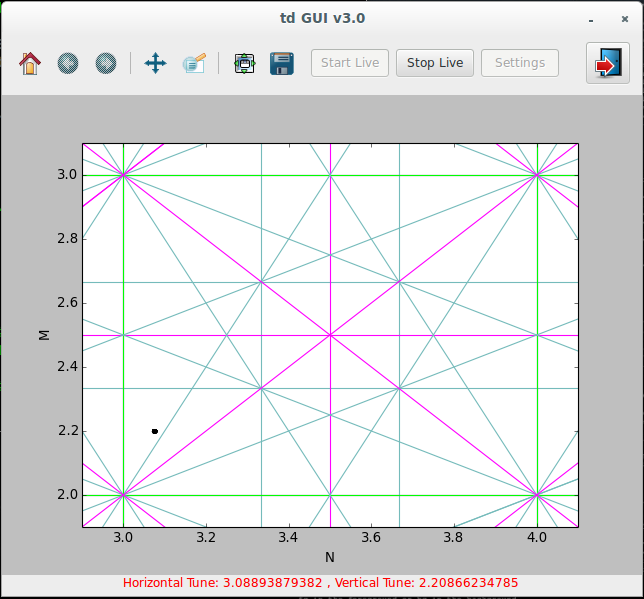
\includegraphics[width=150pt]{main.png}}
\end{center}
Continue with stuff and things blah blah blah blah blha blah blah
\subsection{Developement}
The program is written in Python and completely open source. This provided the opportunity to integrate with EPICS (Experimental Physics and Industrial Control System) through a special python package called PyEpics and build a GUI system using wxPython to make the program simple to use. Much of the program also relies heavily on numpy and matplotlib packages available for Python.

The biggest feature of the program is a 'live mode' option that is able to give the current tune position numerically and graphically. Using the proper epics channels, the program is able to grab the four values it needs to calculate the non integer tune: the RF cavity frequency, the harmonic number, and the horizontal and vertical betatron oscillation frequencies. The program can check and update the tune several times a second, but in order to have the visual display updated, a threading process was used to avoid having the GUI freeze up while in live mode. The threading process is able to do all the processing and updating of the matplotlib graph, continously updating the working point on the plot.

\subsection{Customizability}
Various customizability options are available for the program. Changing color settings, removing certain resonance lines, and adjusting for mirrored tunes are just some features available for the user. Being able to display phase advance resonance lines is another unique feature included in the program.

Aside from accelerators having to position their working points away from resonane lines, they must also consider the phase advanced resonance lines as these are much more powerful and dangerous to approach with a working point. Given the number of unit cells for the machine, the program is able to display a tune diagram with the phase advance resonance lines along with the working points. This feature can complement the live mode option available with the program. If an operator wants to move the working point and cross resonance lines, the program can be used as a visual guide in order to avoid the phase advanced resonance lines (colored in red in figure 1) which will more than likely kill the beam.
\begin{center}
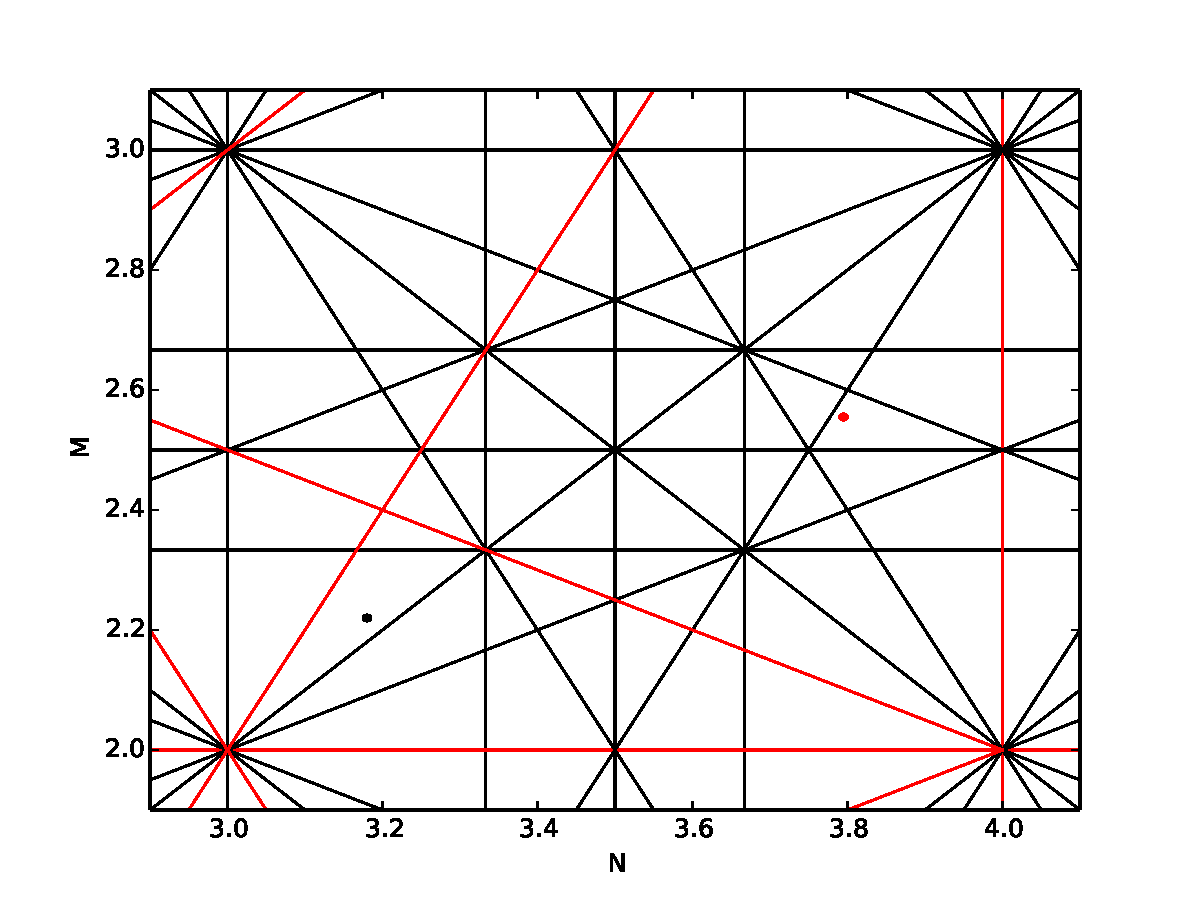
\includegraphics[width=200pt]{image.pdf}
\end{center}
Figure 2: Tune resonance diagram displaying phase advance lines (4 unit cells) for the MLS

\subsection{Future Improvements}
The program's availability on github\cite{Note1} allows for updates and improvements to be added in the future. Because of a lack of time, some improvements and features will be added at a later date. One of these improvements is the amount of CPU power the program uses when running in live mode. The problem stems from the matplotlib package having to constantly update the graph/plot several times a second; this process ends up consuming a lot of CPU power and eventually slows down the program significantly. Aside from this, there are minor improvements that will be added in occasionally depending on the amount of free time available.


\section{Streak Camera}
A streak camera is a device used to take pictures of very fast light phenomena. The resulting images however are not like that of a typical camera, but instead are given in a plot of intensity vs time vs position.
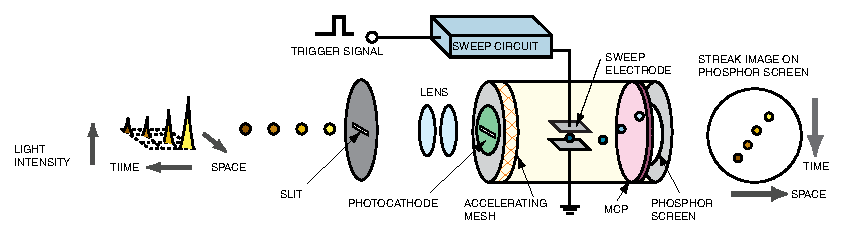
\includegraphics[width=250pt]{streakdiagram.pdf}
Figure 3: Streak camera operational principals\cite{Note2}. \\

How the camera actually works is illustrated in figure 3. Radiation enters the camera's slit as photons with varying intensity emitted from the electrons in the beam; it then goes through some lens before hitting a photocathode. The photocathode converts the photons into a certain number of electrons proportional to the intensity of the light. The accelerating mesh then accelerates the electrons towards the phosphor screen. The electrons then go through a sweeping electric field that deflects them at slightly different angles vertically depending on the arrival time of the electrons. The micro channel plate then multiplies the electrons several thousand times in order for their impact on the phosphor screen to be detectable. Finally, the electrons hit the phosphor screen and are transformed back into photons; their positions on the screen depend on their arrival time at the sweeping electrode. The earliest electrons are deflected to the top of the screen and the latest electrons are at the bottom of the screen; this turns the vertical axis into a time axis and allows the measuring of the bunch length for the beam either with FWHM or sigma.

\subsection{Setup}
The setup of the streak cameras proved to be quite a challenge. The cameras had to be on top of a specific optical table that was positioned behind and above the beamline; this required an optical path that would provide six degrees of freedom.
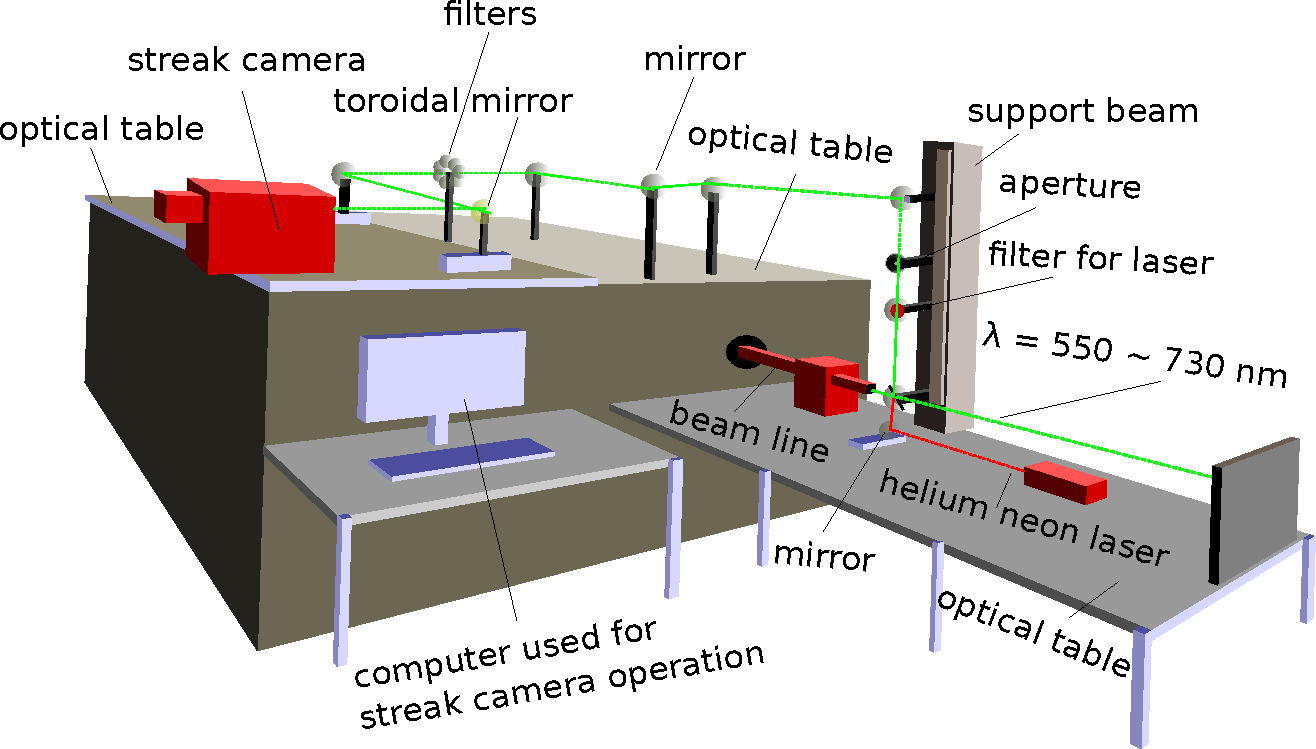
\includegraphics[width=250pt]{diagramtext.pdf}
Figure 4: Rough diagram of stream camera setup \\

The very first thing done when setting up the optical paths was to align a helium neon laser with the beam using a splitter. Beamtime is expensive and not always available, but having a laser that is perfectly aligned with the beam allowed us to continue setting up the optical paths using the laser instead of the beam. The first piece along the optical path is a bandpass filter lens which allows wavelengths between xxx and xxx nm; this is also the wavelength range of the laser. However, in order to have the synchrotron and undulator radiation pass through this filter, the undulator gap must be manually moved which shifts the peaks in figure 5 into the range of our filter. Next we pass through an aperture that is used to help focus the beam before finally hitting a plane mirror at the top of our vertical beam.
\begin{center}
\fbox{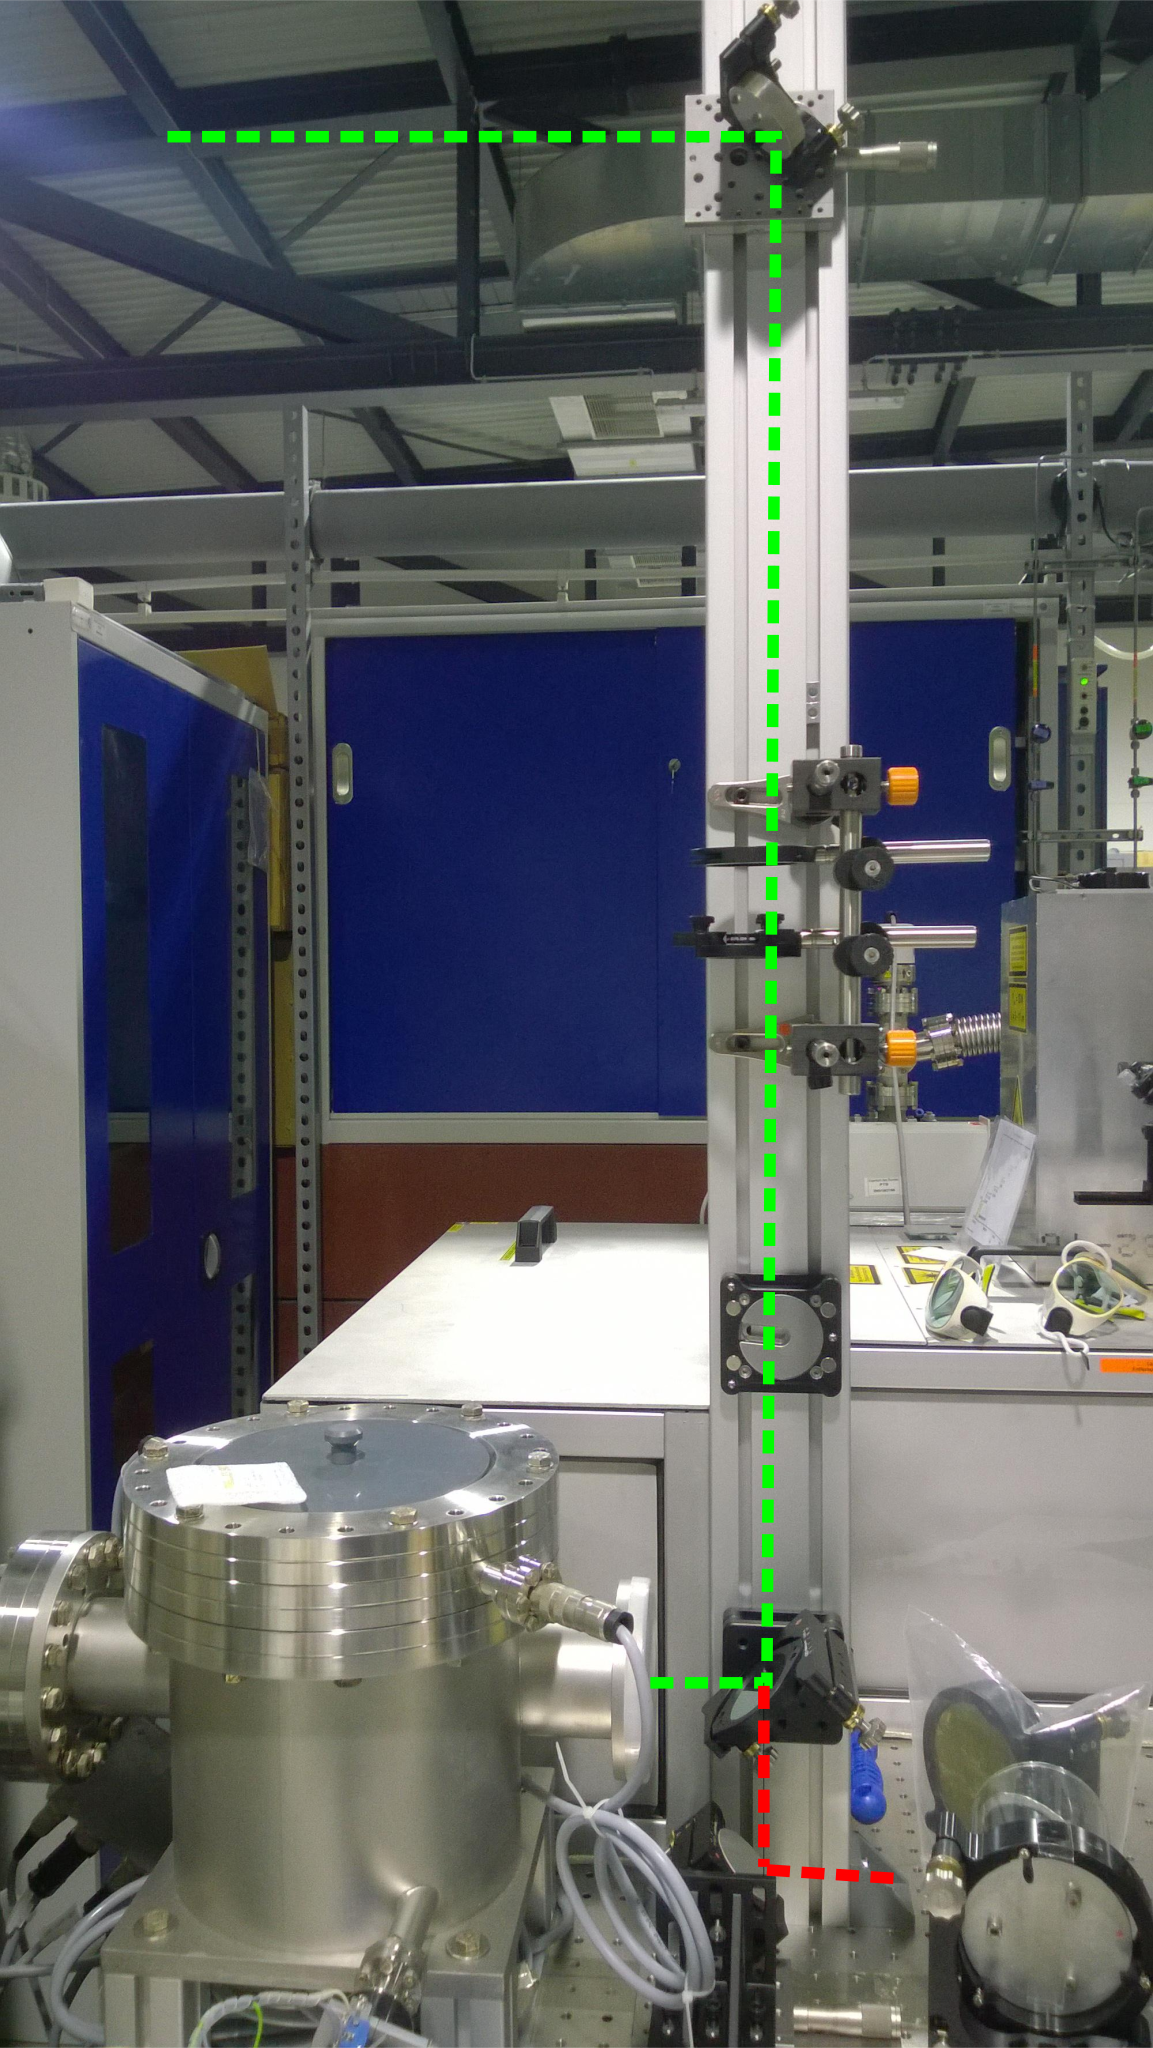
\includegraphics[width=150pt]{verticalbeam.pdf}}
\end{center}
\begin{center}
Figure 6: Vertical beam setup
\end{center}

The next thing we did is setup the horizontal optical table that went directly into the two new streak cameras



\subsection{Operation}
The citation style for AIP journals is:
\begin{itemize}
\item 
numerical (default style), 
\item
author-year, and
\item
numerical author-year,
\end{itemize}
the latter two styles being only allowed for \textit{Chaos} or \textit{J. Math. Phys.}

The familiar numerical citations and numbered bibliography are the default for most journals: 
citations are superscript numbers, and the (numbered) bibliographic entries appear in the order cited. 

Author-year citations are only allowed for 
\textit{Chaos} or \textit{J. Math. Phys.}, with citations given in author-and-year format. 
Bibliographic entries are sorted by alphabetical order of first author's surname, then by year. 

Numerical author-year citations 
(only allowed for \textit{Chaos} or \textit{J. Math. Phys.}) 
are superscript numbers, just like numerical citations, 
but the bibliographic entries are sorted like the author-year entries and are numbered. 
This means that the first citation will not necessarily be~1.

To obtain the numerical style, simply accept the default, or supply a class option of \texttt{numerical}:
\begin{verbatim}
\documentclass[aip,numerical]{revtex4-1}
\end{verbatim}
For author-year citations for \textit{Chaos} or \textit{J. Math. Phys.}, 
you may specify the \texttt{author-year} option:
\begin{verbatim}
\documentclass[aip,author-year]{revtex4-1}
\end{verbatim}
Each of the above two options are part of standard \revtex.

To obtain numerical author-year citations 
for \textit{Chaos} or \textit{J. Math. Phys.}, 
give the author-numerical option:
\begin{verbatim}
\documentclass[aip,author-numerical]{revtex4-1}
\end{verbatim}
Note that the \texttt{author-numerical} option is not part of standard \revtex\, so use of it
outside of the AIP substyles may not have any effect. 

\subsection{Problems for the Future}
There are two commonly used formats for an article you may write. 
One will comply with the manuscript submission formatting requirements of the editorial office of the journal you are submitting to.
The other will emulate the format of your article in the published journal itself. 

For journal submission, accept the default, or you may specify the \texttt{preprint} option:
\begin{verbatim}
\documentclass[aip,preprint]{revtex4-1}
\end{verbatim}
To emulate the formatting of the journal, specify the \texttt{reprint} option:
\begin{verbatim}
\documentclass[aip,reprint]{revtex4-1}
\end{verbatim}
Note that emulation is not by any means complete: the fonts used will differ, and therefore
the length of the article will not represent an accurate estimate. 
Other details may also differ. 

A summary of class options of interest to AIP authors appears in Table~\ref{tab:options}.

\section{Conclusion}
test test test

\begin{table}
\caption{\label{tab:options}Other class options}
\begin{ruledtabular}
\begin{tabular}{ll}
\textbf{Function} & \textbf{class option} \\
\multicolumn{2}{l}{\textit{Citation and References}}\\
superscript numbered&\texttt{numerical}\footnotemark[1]\textsuperscript{,}\footnotemark[2]\\
author-year&\texttt{author-year}\footnotemark[3]\\
numbered author-year&\texttt{author-numerical}\footnotemark[3]\\
%
\multicolumn{2}{l}{\textit{Format}}\\
journal submission&\texttt{preprint}\footnotemark[1]\\
journal emulation&\texttt{reprint}\\
\end{tabular}
\end{ruledtabular}
\footnotetext[1]{Default option.}%
\footnotetext[2]{Standard}%
\footnotetext[3]{Only allowed for \textit{Chaos} or \textit{J. Math. Phys.}}%
\end{table}



\begin{thebibliography}{9}\label{sec:TeXbooks}%
\bibitem{Note1}
Source code can be found on the following github page: \url{https://github.com/levondov/TuneResonancePython}.
%
\bibitem{Note2}
Hamamatsu,
\emph{Guide to Streak Cameras}
(HAMAMATSU PHOTONICS K.K., Hamamatsu City, Japan, 2008)
\url{http://www.hamamatsu.com/resources/pdf/sys/e_streakh.pdf}.
%
\bibitem[Lamport(1996)]{LaTeXman} 
L. Lamport, 
\emph{\LaTeX\, a Document Preparation System} 
(Addison-Wesley, Reading, MA, 1996).
%
\bibitem[Goossens(1994)]{Compan} 
M. Goosens, F. Mittelbach, and A. Samarin, 
\emph{The \LaTeX\ Companion} 
(Addison-Wesley, Reading, MA, 1994).
%
\bibitem[Knuth(1986)]{TeXbook} 
D. E. Knuth, 
\emph{The \TeX book} 
(Addison-Wesley, Reading, MA, 1986). 
%
\bibitem[Kopka(1995)]{Guide} 
H. Kopka and P. Daly, 
\emph{A Guide to \LaTeXe} 
(Addison-Wesley, Reading, MA, 1995).
%
\bibitem[Goossens(1997)]{CompanG} 
M. Goossens, S. Rahtz, and F. Mittelbach, 
\emph{The \LaTeX\ Graphics Companion} 
(Addison-Wesley, Reading, MA, 1997).
%
\bibitem[Rahtz(1999)]{CompanW} 
S. Rahtz, M. Goossens \emph{et al.},
\emph{The \LaTeX\ Web Companion} 
(Addison-Wesley, Reading, MA, 1999).
%
\end{thebibliography}

\end{document}

